\chapter{Context}\label{ch:context}

Dynatrace Ltd.\footnote{\url{https://www.dynatrace.com/}}, a company specializing in software monitoring, maintains a project called Dynatrace Operator\footnote{\url{https://github.com/Dynatrace/dynatrace-operator}} (DTO).
As stated before, an operator is a system, which runs inside a Kubernetes cluster and communicates with its API.
The DTOs purpose is to communicate with the Kubernetes API in such a way, to deploy OneAgents and ActiveGates in a Kubernetes cluster.
Furthermore, it uses webhooks to add an init-container, containing an OneAgent installation, to scheduled pods, in order to monitor them as well.

\textbf{OneAgents and ActiveGates}~\cite{oneagents,activegates} are Dynatrace proprietary software systems.
The Dynatrace OneAgent~\cite{oneagents} is a software system to monitor other systems and collect metrics of them.
These metrics can range from memory or cpu usage to more complex ones such as network connections or amount of specific function calls.
Two different kinds of OneAgents exist, a host agent and a special agents.
The host agents purpose is to monitor the host of any given system, for example, a server on which a web application is deployed on.
Then, for different technologies, different special agents exist.
A special agent's purpose is to monitor an application, such as the web application mentioned earlier.

An ActiveGates~\cite{activegates} main purpose is to act as a proxy between OneAgents and the Dynatrace cluster.
It can be used to buffer information sent by a OneAgent inside a local network, before uploading it to the main Dynatrace cluster.
Furthermore, it can be used to monitor cloud centric technologies, such as AWS, Kubernetes, Openshift, or other cloud systems.

The DTO is released on a number of ways.
First, the GitHub page itself, in which updated manifests, an updated Helm chart and a new index for these charts are uploaded to.
In addition to the mentioned artifacts, a changelog is also published.
Then, it is released to six different marketplace.
Four of which use one proprietary format to create a marketplace listing, one uses a second proprietary format, while the final one uses a third proprietary format.
Two of the four marketplaces have different rules how this marketplace listing has to look like, although they use the same file format.

The four marketplaces using the ClusterServiceVersion (CSV) format are called RedHat Marketplace (RHMP), certified-operators, community-operators, and community-operators-prod.
All of which operated, or to some degree maintained, by RedHat.
RHMP, certified-operators, and community-operators-prod all create listing which be found in OpenShift.
The remaining community-operator release creates a listing for the Kubernetes OLM deployment.
Finally, RHMP and certified-operators use one set of validation rules for the listing, while the other two use a similar, but different one.

It could be argued that the name ClusterServiceVersion was specifically chosen to annoy developers working with it.
As everytime a problem is searched for in a search engine, the results are usually about the much more common CommaSeperatedValues (CSV) format.
How this issue was not noticed by RedHat developers when naming this format is a question out of scope of this thesis and further research is required.

The fifth marketplace mentioned earlier is the Google Cloud Marketplace (GCM).
It is used to automatically deploy an operator on a Google Kubernetes Engine (GKE) Kubernetes cluster, analogous to RedHat's marketplaces, which deploy an operator on an OpenShift cluster.
Google's marketplace also uses a proprietary format for its listing, which is conveniently completely different to the CSVs Redhat uses.
In the same manner, the sixth and last marketplace, Rancher, use a proprietary format as well.
Similar to the format used by the GCM listing, it is also completely different.

Finally, all the mentioned marketplaces have different release mechanisms.
Some of them similar, some of them entirely distinct.
As is shown in a later section, RHMP and certified, as well as community-operators and community-operators-prod, there are enough similarities so that basically only the upload target has to change.
For the others, the release process is so dissimilar, that there is no common denominator.

Before the DTO is released, however, it must be tested.
At the time of conducting this research, the project has only been tested using unit tests, with some attempts of using integration tests.
A lot of E2E testing is also done by teams specialized in writing E2E tests, in cooperation with the development team.

Integration tests are still an issue.
First, integration tests can make sure that different parts of the DTO are working well together.
Unit-tests can be used to find faults in the code, but they do not test different routines working together, whereas integration tests do.
On the other hand, they give confidence to the development team, which is responsible for releasing the DTO in a functioning state.
In order to test the DTO appropriately, a tool is implemented as part of this thesis to organize and execute integration tests.
Due to the nature of an operator, running in big clusters, it uses the techniques of similarity testing mentioned in chapter~\ref{ch:introduction} to select a manageable amount of tests to run.
The system to select and manage tests has been called Dynamic Testing Framework (DTF).

Both systems are using the Concourse CI/CD system in one way or the other.
The release pipeline is built to run entirely in it, as a pipeline that can be executed either manually or automatically to create a functioning release.
The (DTF) generates a pipeline configuration for Concourse, with the selected tests that are to be run.

\section{Architecture}\label{sec:architecture}

\begin{figure}[h]
    \centering
    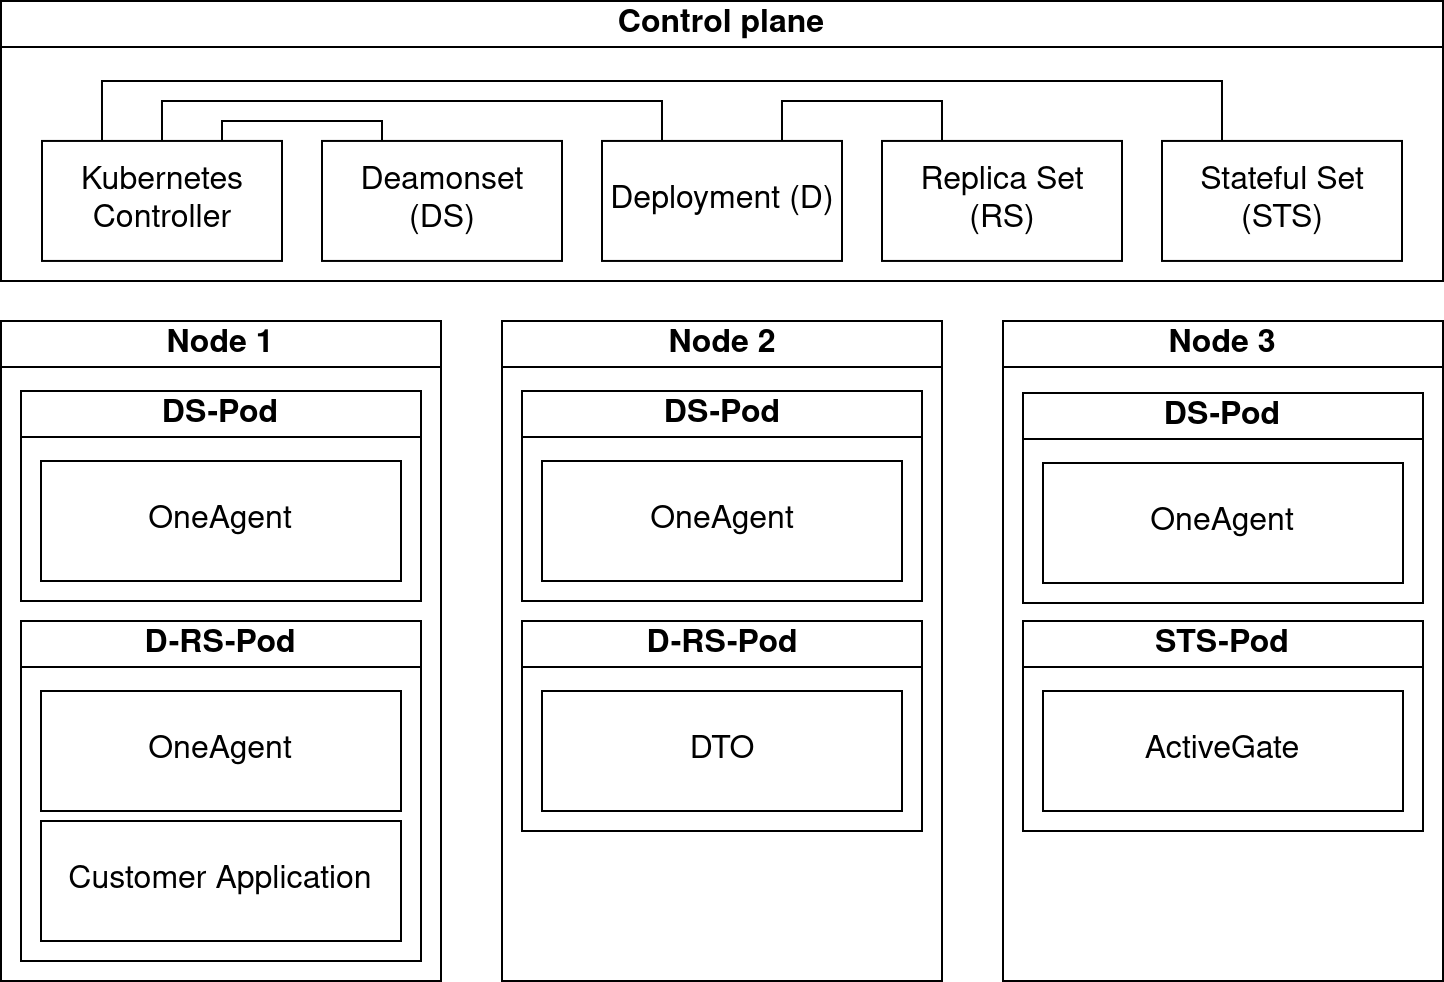
\includegraphics[width=\textwidth]{img/context/kubernetes}
    \caption{Kubernetes architecture}
    \label{fig:kubernetes-architecture}
\end{figure}

In figure~\ref{fig:kubernetes-architecture}, an exemplary setup of all the previously discussed technologies can be seen.
The Kubernetes controller is aware of all its resources.
In this example, the relevant resources are deamonsets, deployments and the replicasets they control, and stateful sets.
If the DTO is configured as such, it deploys OneAgents monitoring the host, using a daemonset, so they are deployed once on every node.
Then it creates a statfulset which deploys an instance of an ActiveGate.
Finally, the webhook of the DTO injects scheduled customer pods with application specific OneAgents.

This setup is one of the simplest setups that is possible while still being representative of real world example.
It becomes apparent why a complex test setup is needed, since the environment the DTO runs in is equally complex.
A Kubernetes cluster must be created and setup for it to run in.
Example applications must be deployed and configured for correct injection.

\begin{figure}[H]
    \centering
    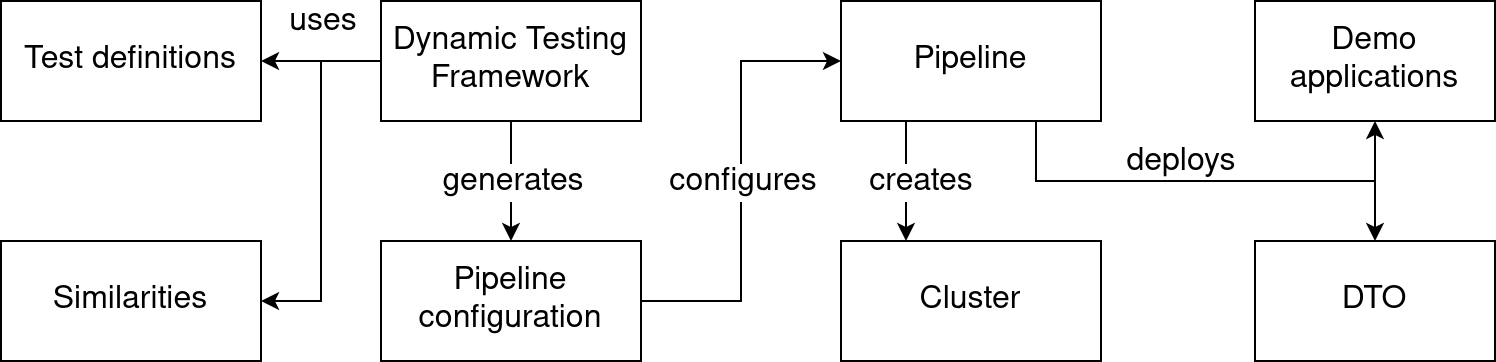
\includegraphics[width=\textwidth]{img/context/dtf}
    \caption{Dynamic Testing Framework workflow}
    \label{fig:dtf-workflow}
\end{figure}

In figure~\ref{fig:dtf-workflow} the general workflow of the DTF is shown.
Test definitions and how similarities are used are explained in section~\ref{subsec:test-definitions} and section~\ref{subsec:similarities}.
The DTF uses both to generate a pipeline configuration for Concourse.
This configuration can then be applied to a running Concourse instance and started.
The idea is, that this pipeline then creates a cluster, configures it and deploys the DTO as well as needed applications on it.
Further tasks of this pipeline can then check for specific states when applying different DTO configurations.
After all tests succeeded, a second pipeline, the release pipeline, can be triggered.

\begin{figure}[H]
    \centering
    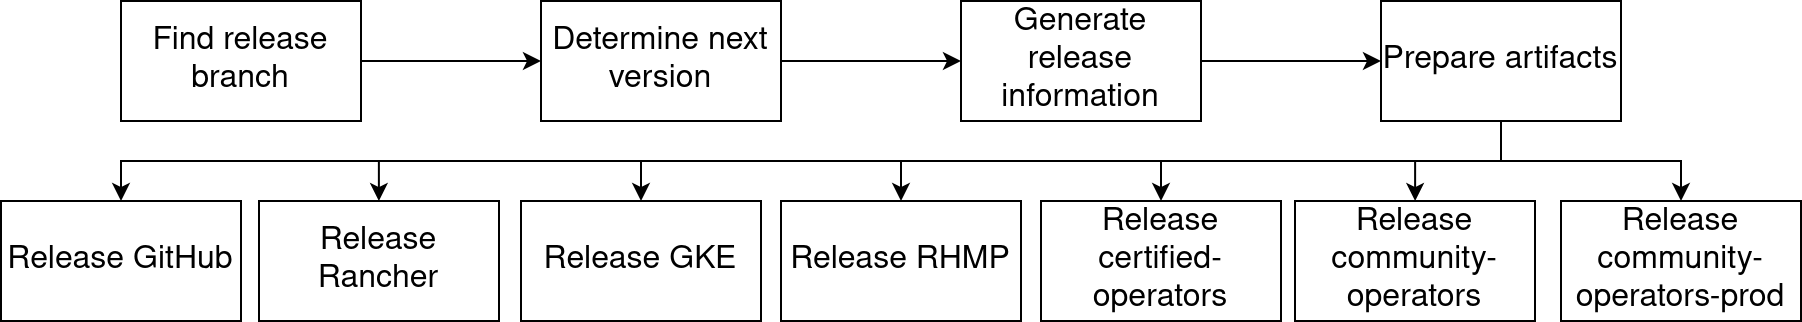
\includegraphics[width=\textwidth]{img/context/release pipeline}
    \caption{Release pipeline}
    \label{fig:release-pipeline}
\end{figure}
